%
% teil5.tex -- 3D-Drucker
%
% (c) 2020 Prof Dr Andreas Müller, Hochschule Rapperswil
%
% !TEX root = ../../buch.tex
% !TEX encoding = UTF-8
%
\section{Mechanismen aus dem 3D-Drucker
\label{geradlinig:section:mechanismen_aus_dem_3d_drucker}}
\kopfrechts{Mechanismen aus dem 3D-Drucker}
Um das Verständnis dieser Mechanismen zu vertiefen, lohnt es sich,
diese selbst nachzubauen.
Der Peaucellier-Lipkin-Mechanismus wurde bereits 
für den 3D-Druck konstruiert und öffentlich 
zugänglich gemacht~\cite{thingiverse}.
Die Mechanismen können grundsätzlich aus einfachen Gelenken und Bolzen 
aufgebaut werden, wie sie in Abbildung~\ref{fig:3dprint_mech} 
dargestellt sind.
Da die Gelenke teilweise unterschiedlich übereinander angeordnet werden, 
braucht es Bolzen mit unterschiedlichen Längen.
\begin{figure}
    \centering
    \begin{minipage}{0.32\textwidth}
        \centering
        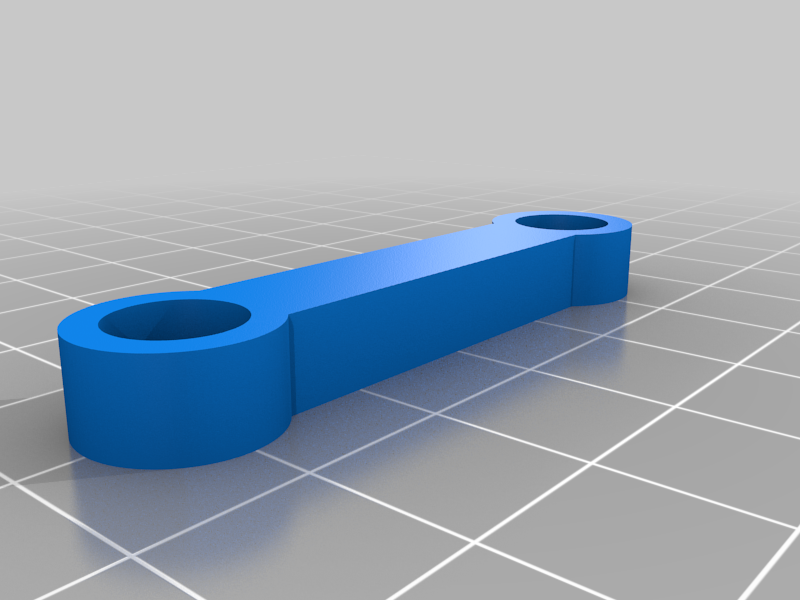
\includegraphics[width=\textwidth]{papers/geradlinig/figures/link_driver.png}
    \end{minipage}
    \hfill
    \begin{minipage}{0.32\textwidth}
        \centering
        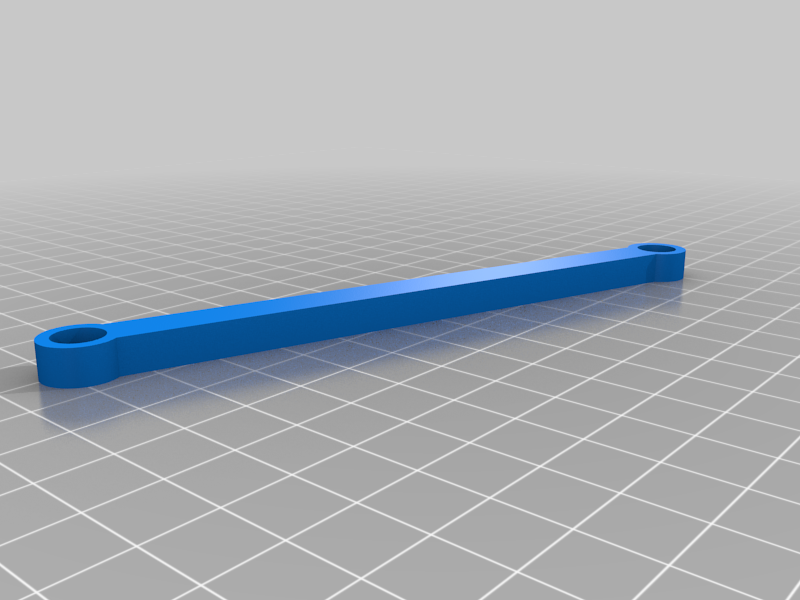
\includegraphics[width=\textwidth]{papers/geradlinig/figures/link_long_lower.png}
    \end{minipage}
    \hfill
    \begin{minipage}{0.32\textwidth}
        \centering
        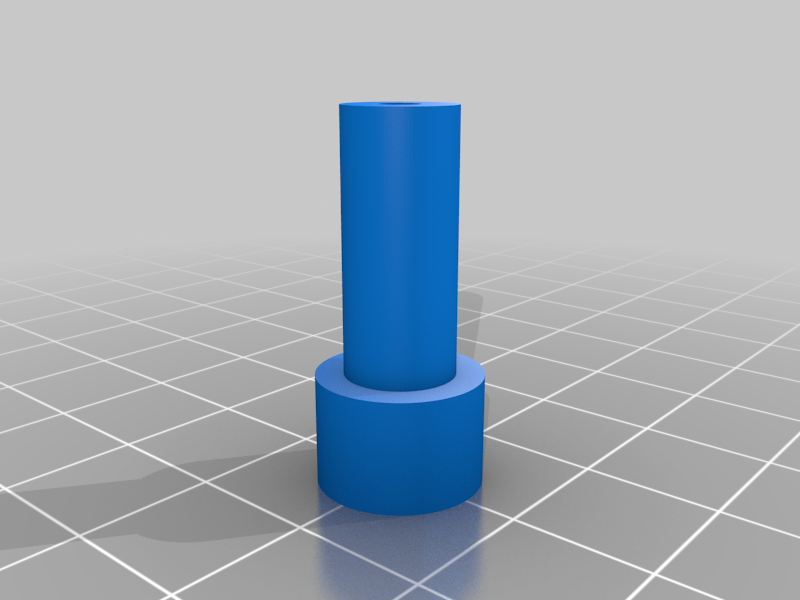
\includegraphics[width=\textwidth]{papers/geradlinig/figures/pin_lower.png}
    \end{minipage}
    \caption{Beispiele für Standardgelenke und Bolzen 
    für den 3D-Druck~\cite{thingiverse}.}
    \label{fig:3dprint_mech}
\end{figure}


Der Mechanismus muss auf einer festen Basis montiert werden.
Dadurch können sich die Bolzen mit möglichst geringer Reibung 
in den Gelenken bewegen.
Die CAD-Kon\-struk\-tion mit der Basis für den Perrolatz-Mechanismus 
ist in Abbildung~\ref{fig:3dprint_cad} dargestellt.
\begin{figure}
    \centering
    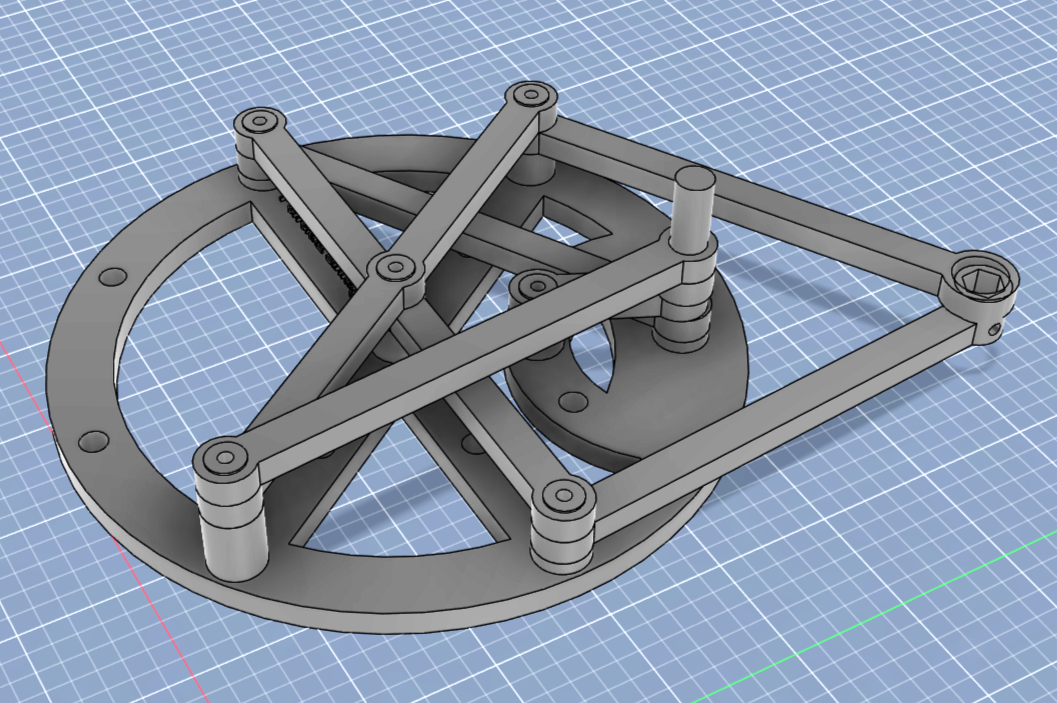
\includegraphics[width=0.9\textwidth]{papers/geradlinig/figures/perrolatz_inversor_v22.png}
    \caption{CAD-Konstruktion des Perrolatz-Mechanismus mit Basis.}
    \label{fig:3dprint_cad}
\end{figure}


Die Konstruktion kann anschliessend mit einem 3D-Drucker hergestellt werden.
Das Ergebnis kann wie in den Abbildungen~\ref{fig:3dprint_perr} 
und~\ref{fig:3dprint_peauc} aussehen.
Das Design wurde so ausgelegt, dass am Gelenkende, wo die 
geradlinige Bewegung entsteht, ein Stift befestigt werden kann.
Die STL-Files beider Konstruktionen sind im 
folgenden Repository zu finden~\cite{github_stl_mechanism}.
Bei einem 3D-gedruckten Mechanismus ist das Spiel der Gelenke 
jedoch vergleichsweise gross.
\begin{figure}
    \centering
    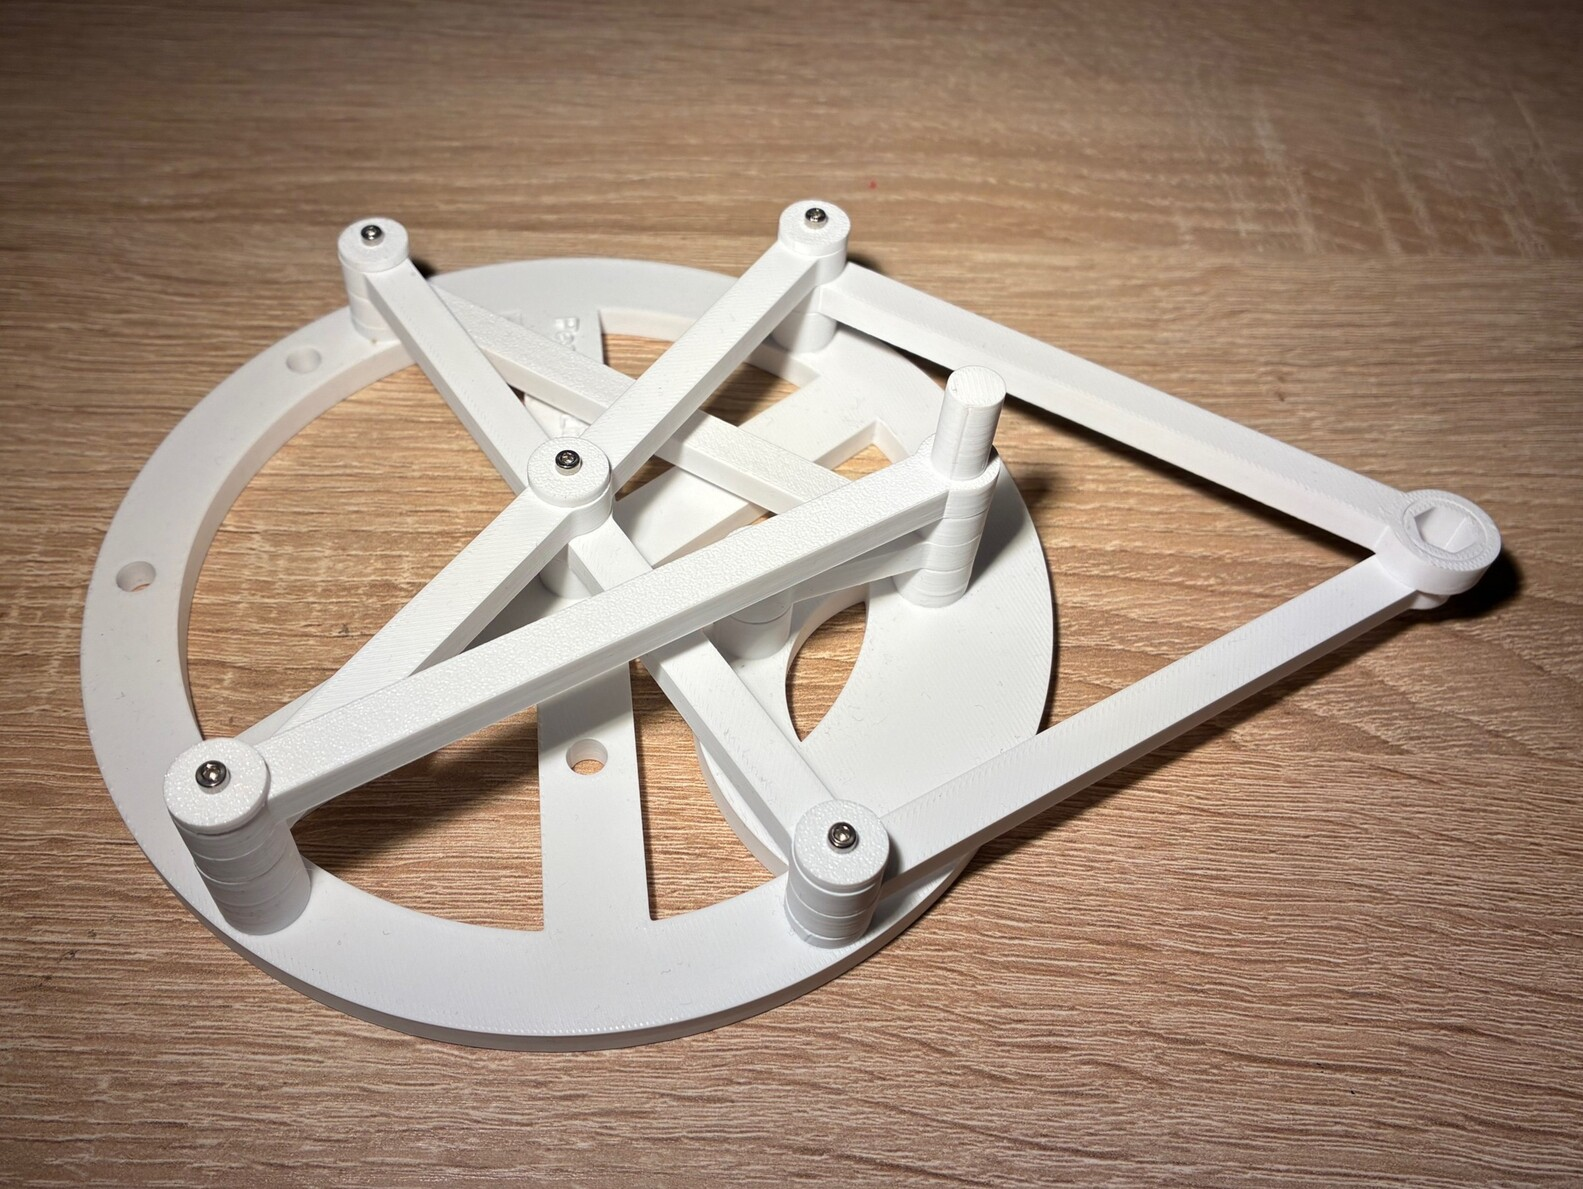
\includegraphics[width=0.9\textwidth]{papers/geradlinig/figures/perrolatz_3dprint-small.jpeg}
    \caption{3D-gedrucktes Modell des Perrolatz-Mechanismus.}
    \label{fig:3dprint_perr}
\end{figure}

Dadurch ist bereits mit blossem Auge erkennbar, dass die Bewegung 
des Ausgangs nicht exakt einer Geraden entspricht.
Sie liegt jedoch trotzdem nahe an einer geradlinigen Bewegung.
Für eine höhere Präzision wäre eine Fertigung aus Metall besser geeignet.
Als einfaches Experiment zur Überprüfung der Funktionsweise eignet 
sich der 3D-gedruckte Mechanismus dennoch gut.
\begin{figure}
    \centering
    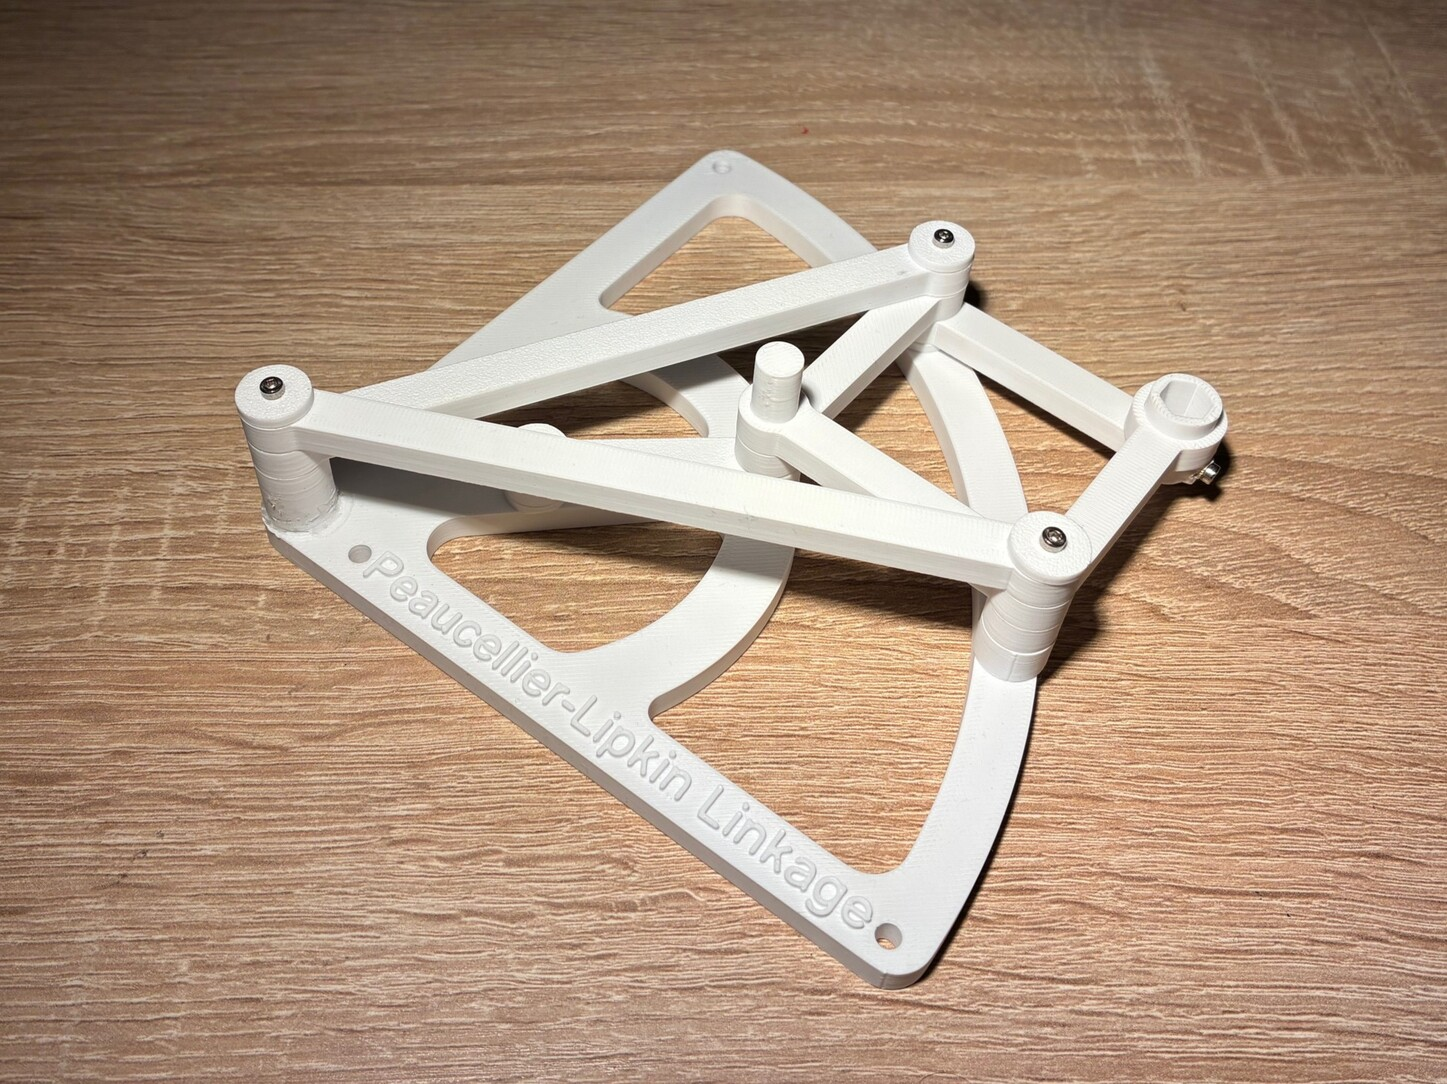
\includegraphics[width=0.9\textwidth]{papers/geradlinig/figures/peaucellier_3dprint-small.jpeg}
    \caption{3D-gedrucktes Modell des Peaucellier-Lipkin-Mechanismus.}
    \label{fig:3dprint_peauc}
\end{figure}

